\documentclass{article}

% if you need to pass options to natbib, use, e.g.:
%     \PassOptionsToPackage{numbers, compress}{natbib}
% before loading neurips_2019

% ready for submission
% \usepackage{neurips_2019}

% to compile a preprint version, e.g., for submission to arXiv, add add the
% [preprint] option:
%     \usepackage[preprint]{neurips_2019}

% to compile a camera-ready version, add the [final] option, e.g.:
     \usepackage[final]{neurips_2019}

% to avoid loading the natbib package, add option nonatbib:
%     \usepackage[nonatbib]{neurips_2019}

\usepackage[utf8]{inputenc} % allow utf-8 input
\usepackage[T1]{fontenc}    % use 8-bit T1 fonts
\usepackage{hyperref}       % hyperlinks
\usepackage{url}            % simple URL typesetting
\usepackage{booktabs}       % professional-quality tables
\usepackage{amsfonts}       % blackboard math symbols
\usepackage{nicefrac}       % compact symbols for 1/2, etc.
\usepackage{microtype}      % microtypography
\usepackage{color}

\usepackage{amsmath,amssymb,amsfonts,amsthm}
\usepackage{graphicx}
\usepackage{bbm}
\usepackage{latexsym}
\usepackage{natbib}
\usepackage{multirow}

\newcommand{\Yten}{\pmb{Y}}
\newcommand{\subs}{\pmb{i}}
\newcommand{\wsu}[2]{#1_{\subs #2}}
\newcommand{\wsup}[2]{#1_{\subs}^{(#2)}}

% Aliases for some of the complicated y-indexing
\newcommand{\ytP}{\wsup{\tilde{y}}{+}}
\newcommand{\ytPM}{\wsup{\tilde{y}}{\pm}}
\newcommand{\ysk}{y_{\subs k}}
\newcommand{\ys}{y_{\subs}}
\newcommand{\ysh}{\hat{y}_{\subs}}
\newcommand{\taus}{\tau_{\subs}}
\newcommand{\lamP}{\wsup{\lambda}{+}}
\newcommand{\lamM}{\wsup{\lambda}{-}}
\newcommand{\lamPM}{\wsup{\lambda}{\pm}}
\newcommand{\gP}{\wsup{g}{+}}
\newcommand{\gM}{\wsup{g}{-}}
\newcommand{\gPM}{\wsup{g}{\pm}}
\newcommand{\factori}[1]{\theta^{(#1)}}
\newcommand{\mus}{\mu_{\subs}}
\newcommand{\musk}{\mu_{\subs k}}

\newcommand{\ms}{m_{\subs}}
\newcommand{\yvs}{\vec{\boldsymbol{y}}_{\subs}}
\newcommand{\yvtP}{\boldsymbol{\tilde{y}}_{\subs}^{(+)}}


% Commands for sampling
\newcommand{\Bess}[1]{\textup{Bessel}\left( #1 \right)}
\newcommand{\Binom}[1]{\textup{Binom}\left( #1 \right)}
\newcommand{\Exp}[1]{\textup{Exp}\left( #1 \right)}
\newcommand{\Gam}[1]{\textup{Gamma}\left( #1 \right)}
\newcommand{\Multi}[1]{\textup{Multinom}\left( #1 \right)}
\newcommand{\Skel}[1]{\textup{Skellam}\left( #1 \right)}
\newcommand{\Pois}[1]{\textup{Poisson}\left( #1 \right)}
\newcommand{\Geo}[1]{\textup{2SGeom}\left( #1 \right)}
\newcommand{\Delt}[1]{\mathbbm{1}\left( #1 \right)}

% Naming Bessel arguments
\newcommand{\besv}{order}
\newcommand{\besa}{coordinate}

% Expectations
\newcommand{\Eq}[1]{\mathbbm{E}_Q\left[#1\right]}
\newcommand{\Vq}[1]{\mathbbm{V}_Q\left[#1\right]}
\newcommand{\Gq}[1]{\mathbbm{G}_Q\left[#1\right]}
\newcommand{\E}[1]{\mathbbm{E}\left[#1\right]}
\newcommand{\V}[1]{\mathbbm{V}\left[#1\right]}
\newcommand{\G}[1]{\mathbbm{G}\left[#1\right]}

\newcommand{\Gqnot}[2]{\mathbbm{G}_{Q_{\backslash #1}}\left[#2\right]}
\newcommand{\Eqnot}[2]{\mathbbm{G}_{Q_{\backslash #1}}\left[#2\right]}

\newcommand{\given}{\,|\,}
\newcommand{\teq}{\!=\!}
\newcommand{\tp}{\!+\!}
\newcommand{\tm}{\!-\!}
\newcommand{\compcond}[1]{\big(#1\given-\big)}

% Spelling naive with the diacritical
\newcommand{\naive}{na\"{i}ve}
\newcommand{\Naive}{Na\"{i}ve}

\newcommand{\TODO}[1]{{\color{red} #1}}

\newtheorem{proposition}{Proposition}


\title{A Variational Approach for Locally Private Inference of Poisson Factorization Models}

\author{} % LEAVE BLANK FOR ORIGINAL SUBMISSION.

% \author{\Name{Alexandra Schofield} \Email{xanda@cs.cornell.edu} \AND
% \Name{Aaron Schein} \Email{aschein@cs.umass.edu} \AND \Name{Zhiwei Steven Wu}
% \Email{zsw@umn.edu} \AND \Name{Hanna Wallach} \Email{hanna@dirichlet.net} }

\begin{document}

\maketitle

\begin{abstract}
  Recent work \cite{schein2018locally} introduces a method for locally private
  posterior inference in Poisson factorization models of count data. This method
  first adds differentially private noise to the sensitive count data and then
  performs noise-aware MCMC inference wherein values of the sensitive data are
  sampled as latent variables. This sampling-based method can be prohibitively
  slow for high-dimensional, large-scale data sets such as text corpora or
  social networks. We improve on this method with a coordinate ascent
  variational inference (CAVI) algorithm to perform locally private inference in
  Poisson factorization efficiently. Our algorithm relies on several new
  properties we prove about the Bessel distribution that may be of independent
  interest. We demonstrate that our algorithm produces a substantial speed
  improvement over the comparable MCMC algorithm in experiments on both
  synthetic and real data.
\end{abstract}

  \section{Introduction}
  % we present a method for privatizing Bayesian inference for Poisson
  % factorization
  % \citep{titsias2008infinite,cemgil2009bayesian,zhou2012augment,gopalan2013efficient,paisley2014bayesian},
  % a broad class of models for learning latent structure from discrete data.
  % This class contains some of the most widely used models in the social
  % sciences, including topic models for text corpora
  % \citep{blei2003latent,buntine2004applying,canny2004gap}, genetic population
  % models \citep{pritchard2000inference}, stochastic block models for social
  % networks \cite{ball2011efficient,gopalan2013efficient,zhou2015infinite}, and
  % tensor factorization for dyadic data
  % \cite{welling2001positive,chi2012tensors,schmidt2013nonparametric,schein2015bayesian,schein2016bayesian};
  % it further includes deep hierarchical models
  % \citep{ranganath2015deep,zhou2015poisson}, dynamic models
  % \citep{charlin2015dynamic,acharya2015nonparametric,schein2016pgds}, and many
  % others. Our method is general and modular, allowing social scientists to
  % build on (instead of replace) their existing derivations and implementations
  % of non-private Poisson factorization. To derive our method, we rely on a
  % novel reinterpretation of the geometric mechanism
  % \cite{ghosh2012universally}, as well as a previously unknown general
  % relationship between the Skellam \citep{skellam1946frequency}, Bessel
  % \citep{yuan2000bessel}, and Poisson distributions; we note that these new
  % results may be of independent interest in other contexts.

  Poisson factorization models are a powerful tool in social science and machine
  learning for understanding data generated by people. For instance, a corporate
  email corpus can surface count data such as interactions between parties,
  counts of words in documents, and logs of events and their participants. However, these data may also encode interactions
  and content that their human generators wish to keep private, which risks the model leaking information specific to a few interactions.
  
  Most existing methods for private inference of exponential family models
  operate in the \emph{central model}
  \citep{park2016private,bernstein2018differentially}, in which a trusted
  aggregator collects all the data and perturbs it to ensure privacy. Recent
  work by \cite{schein2018locally} provides a privacy-preserving method for
  Poisson factorization models in the \emph{local model}, in which individual
  users perturb their own data to ensure privacy without relying on any trusted
  party. The privacy guarantee uses a generalization of local differential
  privacy \citep{warner1965randomized} called \textit{limited-precision local
  privacy}, which allows privacy protection on observations of variable scales
  (e.g. ranging from an entire document to a single word token). A corresponding
  MCMC procedure for inference of Poisson factorization models relies on the
  recharacterization of the traditional data generative process to include the
  addition of perturbation through two-sided geometric noise
  \citep{ghosh2012universally}, with the true data characterized a random
  variable generated using the Skellam and Bessel distributions.
  
  The implementation of this method in prior work of \citep{schein2018locally}
  applies an MCMC approach to iteratively resample the latent variables, such
  that after an initial burn-in period of resampling, these samples may be
  aggregated to estimate the true model parameters. However, this approach to
  private Bayesian Poisson matrix factorization is prohibitively slow for two
  primary reasons. First, it requires sampling from the Bessel distribution,
  which is much slower than sampling for nonprivate Poisson factorization.
  Second, the addition of private noise produces a denser matrix of
  observations, in which no observed zero entry in the data is necessarily a
  true zero in the original data. This addition converts inference from a sparse
  problem, where zero counts could be ignored, to a dense one, where every entry
  in the observed data requires an expensive sampling procedure.
  
  We propose a new mean-field variational inference (VI) procedure to infer
  these models. To do this, we first prove that the Bessel distribution is in
  the exponential family if its parameter $\nu$ is fixed, and that it is the
  optimal Q-distribution for the latent count variables of the true data.
  However, traditional mean-field inference fails, as the resulting expectation
  disrupts downstream inference due to the non-integer value of the expectation
  of the Bessel. We overcome this obstacle by defining the Q-distribution over
  the count to be a delta-spike at the \emph{mode} of the optimal Bessel
  distribution (which is integral, by definition). To show that this mode
  approximation is close to the value obtained using the mean, we prove that the
  absolute difference between the mean and mode of a Bessel distribution is
  bounded by one. Finally, we show that in a synthetic experiment, this method
  converges to reasonable estimates of the true model parameters 20 times faster
  than the MCMC approach.
  
  \section{Background}

  \begin{figure*}[t]
    \centering
    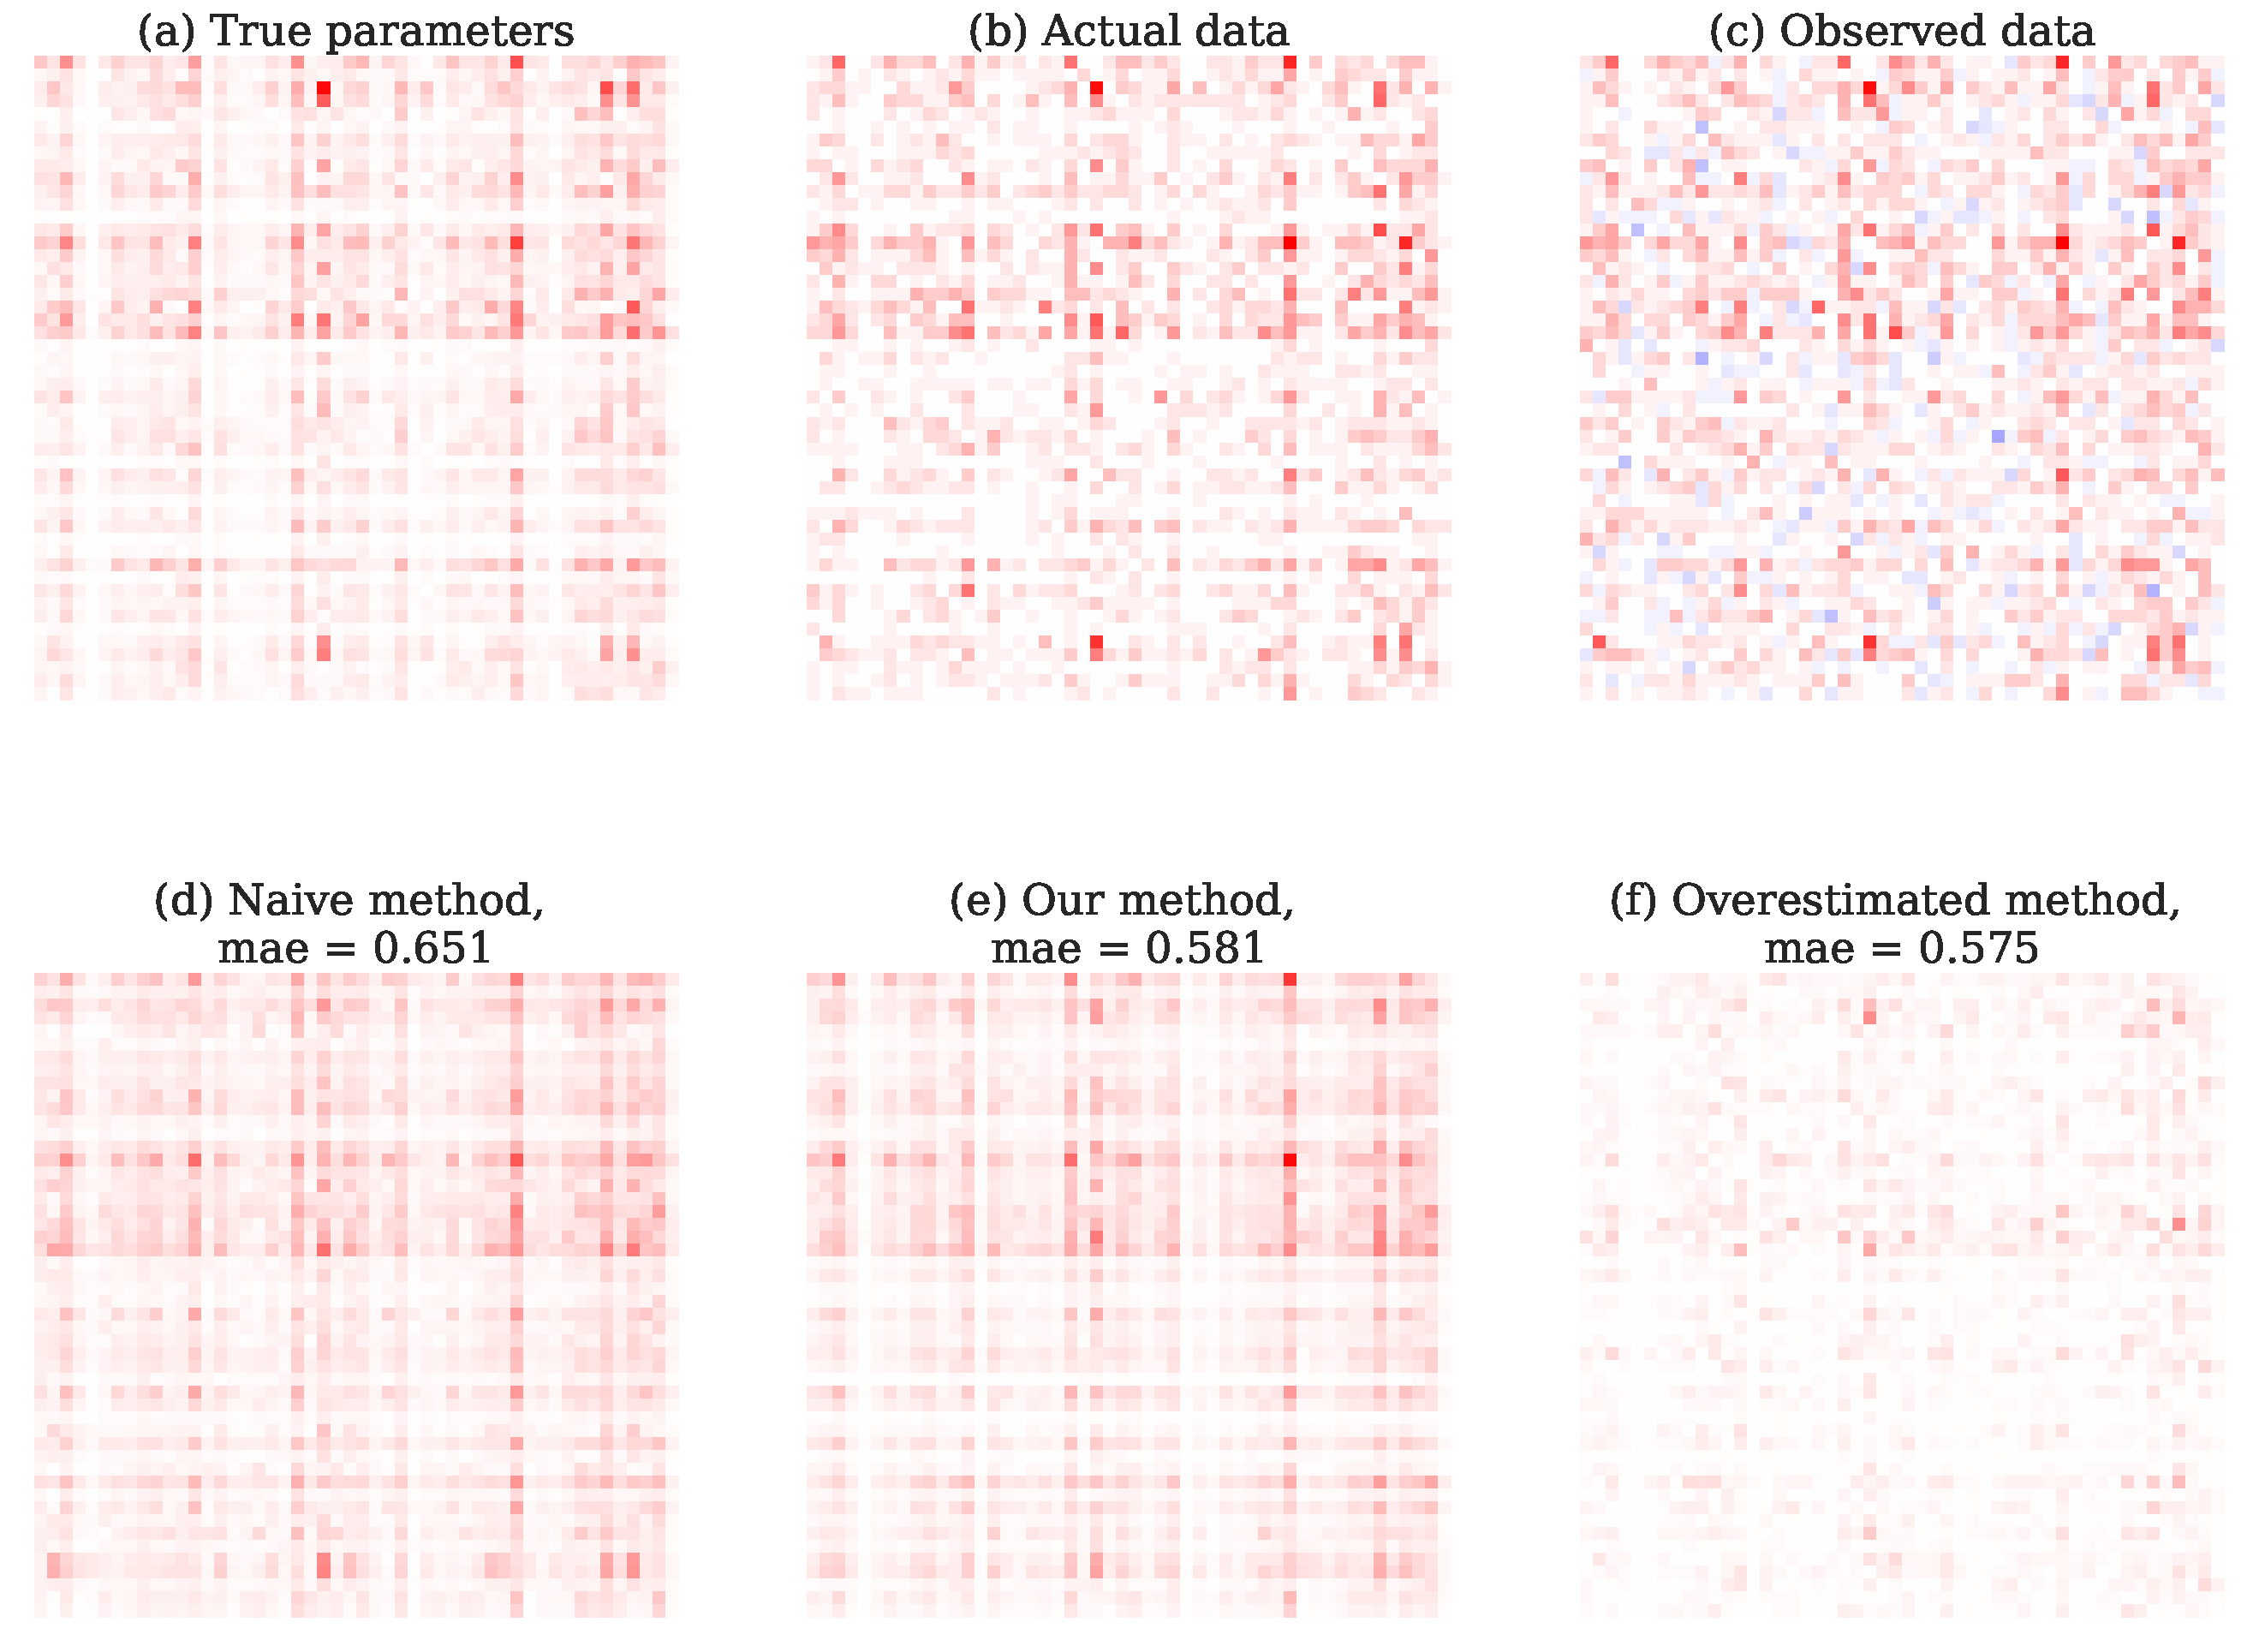
\includegraphics[width=0.95\textwidth]{figures/test_output.pdf}
    \caption{Demonstration of the results of the VI inference process for a
     50-word, 50-document synthetic dataset with 5 latent topics and Gamma prior
     parameters of shape 0.5 and rate 1. The true data parameters (a) are
     recovered better by our inference procedure (e) than by \naive~variational
     inference (d), even though the noisy data (c) is much denser than the true
     data (b).}
    \label{fig:test_output}
  \end{figure*}

  \textbf{Bayesian inference} consists of approximating the posterior
  distribution $P(Z\,|\,Y)$ of latent variables $Z$ given data $Y$. This is
  most often performed using Markov chain Monte Carlo (MCMC) or mean-field
  coordinate ascent variational inference (CAVI). An MCMC inference algorithm
  iteratively re-samples each latent variable from its \emph{complete
  conditional} $z_n \sim P(z_n\,|\,Z_{\backslash n}, Y)$ where $Z_{\backslash
  n}$ denotes the set of all latent variables except $z_n$. CAVI inference
  algorithms specify a factorized variational distribution over latent
  variables $Q(Z) = \prod_n Q(z_n)$ and then optimize its parameters to
  minimize the KL-divergence from it and to the exact posterior. A general
  result is that the optimal factorized $Q(Z)$ consists of $Q(z_n)$ factors
  that are proportional to the geometric expectation of the corresponding
  complete conditional---i.e., $Q^*(z_n) \propto
  \Gqnot{z_n}{P(z_n\,|\,Z_{\backslash n}, Y)}$ where the geometric expectation
  is $\mathbbm{G}[\cdot]=\exp\left(\mathbbm{E}[\ln \cdot]\right)$. In
  practice, CAVI requires orders of magnitude fewer iterations than MCMC to
  converge and is easier to adapt to large-scale streaming data settings.
  
  \textbf{Poisson factorization}
  \citep{titsias2008infinite,cemgil2009bayesian,zhou2012augment,gopalan2013efficient,paisley2014bayesian}
  is a broad class of models for learning latent structure from discrete data,
  containing many of the most widely used models in the social sciences.
  including topic models for text corpora
  \citep{blei2003latent,buntine2004applying,canny2004gap}, population models
  for genetic data \citep{pritchard2000inference}, stochastic block models for
  social networks
  \citep{ball2011efficient,gopalan2013efficient,zhou2015infinite}, and tensor
  factorization for dyadic data
  \citep{welling2001positive,chi2012tensors,schmidt2013nonparametric,schein2015bayesian,schein2016bayesian}.
  It further includes deep hierarchical models
  \citep{ranganath2015deep,zhou2015poisson}, dynamic models
  \citep{charlin2015dynamic,acharya2015nonparametric,schein2016pgds}, and many
  others.
  Poisson factorization assumes that each observed count $\ys$ is a Poisson
  random variable---$\ys \sim \Pois{\mus}$---with unknown rate parameter $\mus$
  that is a deterministic function of shared model parameters. We use the
  multi-index notation $\subs$ for generality; in the special case of Poisson
  \emph{matrix} factorization, each count is indexed by a row and a
  column---e.g., $\subs \!=\! (d, v)$---and its latent rate is defined as the
  dot product of corresponding row and column parameters---i.e., $\mus \teq
  \mu_{\subs} \teq \boldsymbol{\theta}_d^{\top} \boldsymbol{\phi}_v$. In many
  cases, the latent rate is defined to be a \emph{linear} function of shared
  model parameters---i.e., $\mus = \sum_{k=1}^K \musk$, where $\musk$ is a
  function of latent parameters specific to latent component $k$. In Poisson
  matrix factorization, we define $\musk$ as the product of the latent
  parameters associated with $\subs = (d, v)$, or $\musk =
  \theta_{dk}\phi_{kv}$.
  
  \textbf{MCMC for Poisson factorization.} When the latent rate is a linear
  function, the observed count can be interpreted as the sum of latent
  sub-counts---i.e., $\ys = \sum_{k=1}^K \ysk$---where each sub-count is an
  independent Poisson random variable $\ysk \sim \Pois{\musk}$. The first step
  in MCMC inference is to sample the vector of sub-counts $\yvs \teq
  \left(\ysk\right)_{k=1}^K$ from its complete conditional, which is a
  multinomial whose priors are determined by $\mus$, the product of the
  parameter matrix $\theta^{(d)}$:\looseness=-1
  \begin{equation}
  \label{eqn:multinom}
  \compcond{\yvs} \sim \Multi{\ys,\, \boldsymbol{\mu}_{\subs}}
  \end{equation}
  where $\boldsymbol{\mu}_{\subs}\teq \left(\musk\right)_{k=1}^K$. The
  multinomial distribution is often parameterized with a \emph{probability}
  vector $\boldsymbol{p}_{\subs}$. In this paper, we parameterize it using a
  \emph{proportionality} vector $\boldsymbol{\mu}_{\subs}$ which leaves implicit
  the normalization step--i.e., $p_{\subs k} = \frac{\musk}{\sum_{k'=1}^K
  \mu_{\subs k'}}$. Conditioned on samples of the sub-counts, updates to the
  other latent variables are model-specific---i.e., depend on the particular
  structure of the rate function and the priors over the parameters. However,
  our derived approach applies to all models with a linear rate $\mus$. 
  
  \textbf{CAVI for Poisson factorization.} The optimal variational family for
  $\yvs$ is proportional to the geometric expectation of its complete
  conditional (given in Equation~\ref{eqn:multinom}) and equal to:
  \begin{align}
  Q^*\left(\yvs\right) 
  &= \Multi{\yvs; \ys,\, \Big(\Gq{\musk}\Big)_{k=1}^K}
  \end{align}
  The geometric expectations $\Gq{\musk} = e^{\Eq{\ln \musk}}$ can be understood
  as messages from the factors $Q(\musk)$ in the context of a message-passing
  algorithm between variational parameters. In standard cases, these
  expectations are available in closed-form. The factors $Q(\musk)$ depend in
  turn on messages from $Q(\yvs)$ expressed via the expectation of $\ys$:
  \begin{equation}
      \Eq{\ysk}=\ys\frac{\Gq{\musk}}{\sum_{k'=1}^K \Gq{\mu_{\subs k'}}}.
  \end{equation}
  
  \textbf{Locally private MCMC for Poisson factorization}. In locally private
  Poisson factorization, the true data count $\ys$ is unobserved. Instead, we
  observe a noised version of it $\ytPM = \taus + \ys$ where $\taus \sim
  \Geo{\alpha_{\subs}}$ is a randomizing distribution giving a guarantee of
  differential privacy. Following \cite{schein2018locally}, we use a two-sided
  geometric random variable generated based on privacy parameter $\alpha_{\subs} \in [0,1]$.
  The authors demonstrate that such perturbation mechanism satisfies $(N, N
  \ln(1/\alpha_{\subs}))$-limited-precision local privacy.\footnote{A local
  randomizer $R$ satisfies $(N, \epsilon)$-limited-precision local privacy if
  for any two observations $y,y'\in \mathbb{N}^d$ such that $\|y-y'\|_1\leq N$,
  $R$ satisfies $\Pr[R(y) = r] \leq \exp(\epsilon)\Pr[R(y') = r]$ for any $r$ in
  the output range.} Their protocol in this case proceeds by treating the true data $\ys$
  itself as a latent variable and re-sampling it from its complete conditional.

  To find a variational inference algorithm, we leverage existing equivalent
  characterizations of the generative process for Poisson factorization models
  under differential privacy as provided by \citep{schein2018locally}. We
  consider in this case the variable $\ys$ to be a true observed data point,
  while $\ytPM$ is the observed version with random noise. We treat two-sided
  geometric noise as the difference of two Poisson variables $\gP$ and $\gM$,
  generated with Gamma-distributed priors $\lamP$ and $\lamM$, respectively. We
  define auxiliary variables $\ytP = \ys + \gP$ and $\ytPM = \ys + \gP - \gM$ to
  represent a two-step process of adding the two ``sides'' of the noise function
  as Poisson variables. We introduce another auxiliary variable, $\ms$, to
  describe the minimum of $\ytP$ and $\gM$. The sign of observed variable
  $\ytPM$ is sufficient to determine which variable $\ms$ represents: if $\ytPM
  \leq 0$, then $\ms = \ytP$, and if $\ytPM \geq 0$, then $\ms = \gM$. If $\ytPM
  = 0 = \gM$, both these equations are satisfied.

  The key feature of this variable scheme is that it joins together quantities drawn from
  the Poisson parameters of interest and the noise
  distribution directly in the probability of each $\mus$:
  \begin{equation}
    \compcond{\yvtP} \sim \Multi{\ytP, (\lamP, \mu_{\subs 1}, \dots, \mu_{\subs K})}.
  \end{equation} 
  Here, $\yvtP=(\gP, y_{\subs 1}, \dots, y_{\subs K})$ is a vector of latent
  sub-counts that sum to $\ytP$. The first of these sub-counts, $\gP$, represents
  the positive Poisson noise added to the sensitive data $\ys=\sum_{k=1}^K \ysk$,
  while the latter sub-counts correspond to each latent component in non-private
  Poisson factorization.

To infer LPBPF, one may first infer the sums of Poisson distributions of the
underlying data, then thin them using multinomial and binomial draws. In these
equations, delta functions $\mathbbm{1}\left( \cdot \right)$ describe
mathematical constraints that must be met deterministically by auxiliary variables. Some distributions have their own implicit
delta function: for example, a multinomial distribution $\Multi(\vec{x}; n,
\vec{p})$ implicitly constrains the sum of $\vec{x}$ to be
equal to $n$.

Note that we sometimes write the probability parameters in the multinomial and
binomials as unnormalized vectors instead of proper probability distributions.
Also, $\mu_{\subs} = \sum_k \prod_d
\theta_{i_d,k}^{(d)}$, where $i_d$ is the index into the $d$th dimension of
index vector $\subs$.

This gives the following equation as the full generative process of LPBPF:
\begin{align} 
  P &\left(\gP, \gM, \left(\ysk\right)_{k=1}^K, \ys,
    \ytP, \ytPM, \ms\right) = \notag \\
  &\quad\quad \Pois{\gM; \lamM} \,
    \Pois { \ytP; \lamP \tp \mu_{\subs} }
    \notag \\
  &\quad\quad \text{Binom}\left((\ys, \gP);\, \ytP,(\mu_{\subs}, \lamP)\right) \, \text{Mult}\left(\left(\ysk\right)_{k=1}^K;\, \ys, \Big( \prod_d \theta_{i_d,k}^{(d)} \Big)_{k=1}^K\right) \notag \\
  &\quad\quad \mathbbm{1}\left(\ytPM =
    \ytP - \gM\right) \mathbbm{1} \left( \ms =
    \min\{\ytP, \gM\} \right) .
\label{eq:lpbpfpois}
\end{align}

Another way to describe this process flips the order of generation from the
actual process used in creation of the private data. Here, we describe first
generating $\ytPM$ and minimum $\ms$ as Skellam and Bessel random variables
conditioned on what would have been the priors of $\ytP$ and $\gM$. We then
compute $\ytP$ and $\gM$ via their deterministic relationship and, finally, thin
$\ytP$ into the vector of counts per latent component $\yvtP$ using binomial and
multinomial draws:
\begin{align}
    P &\left(\gP, \gM, \left(\ysk\right)_{k=1}^K, \ys,
    \ytP, \ytPM, \ms\right) = \notag \\
  &\quad\quad \text{Skel}\left(\ytPM;\, \lamP \tp \mu_{\subs},\, \lamM\right)\, \text{Bes}\left(\ms;\, |\ytPM|,\,2\sqrt{\lamM(\lamP+\mu_{\subs})}\right)\notag\\
  &\quad\quad \mathbbm{1} \left(\ytP=\ms\right)^{\mathbbm{1}(\ytPM \leq 0)} \mathbbm{1} \left(\gM=\ms\right)^{\mathbbm{1}(\ytPM > 0)} \mathbbm{1}\left(\ytPM = \ytP - \gM\right)\notag\\
  &\quad\quad \text{Binom}\left((\ys, \gP);\, \ytP, (\mu_{\subs}, \lamP)\right) \,  \text{Mult}\left(\left(\ysk\right)_{k=1}^K;\, \ys, \Big( \prod_d \theta_{i_d,k}^{(d)} \Big)_{k=1}^K\right).
\label{eqn:finalfact}
\end{align}
This second factorization enables direct closed-form inference: unlike in
  Equation \ref{eq:lpbpfpois}, $\ytPM$ can be connected directly to the
  parameters of interest for the latent model, $\musk$, without necessarily
  having a good direct estimate of $\ys$. This last factorization that
  enables us to derive the variational distribution.

  
  \section{Locally private variational inference for Poisson factorization}
  In this section we describe the challenges to deriving CAVI for locally
  private Poisson factorization and sketch our solutions. In CAVI, we look to
  impose a factorized variational distribution over all latent variables which,
  in this case, includes the set of auxiliary variables $\mathcal{A}_{\subs}$
  for each data point mentioned in the last section. The main technical
  challenge lies in finding a variational families for $\ms$ and $\yvtP$ that
  yield a good approximation and closed-form messages to the other factors. We
  discuss our solutions to several challenges presented in inference of a CAVI
  algorithm and our solutions.~\looseness=-1
   
  \subsection{CAVI updates for the variational distribution}
  \label{sec:cavi}
  One challenge of the Skellam and Bessel characterization of our generative
  process is determining the appropriate variational distribution of the
  variable $\ms$. The Bessel distribution itself is not an exponential family
  distribution, which would make it a poor candidate for developing a
  variational distribution. However, we are able to demonstrate that when one of
  the two Bessel parameters, $\nu$, is fixed, a Bessel distribution is
  exponential family. As $nu$ is observed as a function of the privacy level
  $\alpha$, this property is satisfied, so the constrained Bessel distribution
  will be sufficient for inference.

  Towards this, we prove two propositions:
  
  \begin{proposition} (Proven in appendix.) The Bessel
  distribution $m \sim \Bess{\nu, a}$ for fixed $\nu$ is an exponential family
  with sufficient statistic $T_{\nu}(m) \teq 2m \tp \nu$, natural parameter
  $\eta_{\nu}(m)\teq \log(\frac{a}{2})$, and base measure $h_{\nu}(m) \teq
  \frac{1}{m!\Gamma(m\tp\nu\tp 1)}$. \looseness=-1
  \end{proposition}
  
  \begin{proposition} The optimal variational distribution for $\ms$ is a Bessel
  distribution:
  \begin{equation}
  \label{eqn:opt}
  Q^*(\ms) = \Bess{\ms; \, |\ytPM|, 2\sqrt{\Gq{\lamM}\Gq{\lamP \tp \mus}}}.
  \end{equation}
  \end{proposition}

  Equations~\ref{eqn:opt} and~\ref{eqn:opt-multi} provide solutions to the initial
  challenge of deriving a tractable and nearly optimal variational family.\looseness=-1
  Recall that the observed data consists of the difference variables $\ytPM$.
  \begin{equation}
    \label{eqn:var1}
  Q \left( \lamPM, \ms, \ytP, \gPM, \ys, \left(\ysk\right)_{k=1}^K\right) \propto
   \Gq{P(\ytPM, \lamPM, \ms, \ytP, \gPM, \ys, \left(\ysk\right)_{k=1}^K \,|\,-)}.
  \end{equation}
  Because the likelihood (i.e., the Skellam term) in
  equation~\ref{eqn:finalfact} does not depend on any of these latent variables,
  it disappears entirely. Pushing in expectations and applying the results of
  Proposition 1, we can then rewrite the right-hand side of
  equation~\ref{eqn:var1} as a product of optimal variational distributions:
    
  \begin{align}
    \label{eqn:caviopt}
  &\Gq{P(\ms, \ytP, \gP, \gM, \ys, \left(\ysk\right)_{k=1}^K \,|\,\ytPM, \alpha)} = \notag \\
  &\quad \quad \text{Gam} \left(\lamP; \Eq{\gP} + 1, \frac{1}{\alpha} \right) \text{Gam} \left(\lamM; \Eq{\gM} + 1, \frac{1}{\alpha} \right) \notag \\
  &\quad \quad \text{Bes}\left(\ms;\, | \ytPM|,\,2\sqrt{\Gq{\lamM}\Gq{\lamP +\mu_{\subs}}}\right) \notag \\
  &\quad \quad \text{Binom}\left((\ys);\,
  \Eq{\ytP}, \frac{\Gq{\mu_{\subs}}}{\Gq{\lamP} + \Gq{\mu_{\subs}}},
  \right) \notag \\
  &\quad\quad \text{Mult}\left(\left(\ysk\right)_{k=1}^K;\, \Eq{\ys}, \Big(\Gq{ \prod_d \theta_{i_d,k}^{(d)} }\Big)_{k=1}^K\right) \notag \\
  &\mathbbm{1} \left(\ytP=\ms\right)^{\mathbbm{1}(\ytPM \leq 0)} \mathbbm{1} \left(\gM=\ms\right)^{\mathbbm{1}(\ytPM > 0)} \mathbbm{1}\left(\ytPM = \ytP - \gM\right).
  \end{align}

  \subsection{Modifications for closed-form inference}

  Two expectations in Equation \ref{eqn:caviopt} do not have an analytic form:
  \begin{align}
  \label{eqn:geomterm_1}
  &\Gq{\lamP + \mu_{\subs}} = \exp\left(\Eq{\ln \left(\lamP
    + \sum_{k=1}^K \prod_d \theta_{i_d,k}^{(d)} \right)}\right) \\
  \intertext{and}
  \label{eqn:geomterm_2}
  &\Gq{\mu_{\subs}} = \exp\left(\Eq{\ln \left(\sum_{k=1}^K \prod_d \theta_{i_d,k}^{(d)} \right)}\right);
  \end{align}
  however, both can be very closely approximated using the delta
  method~\citep{ver2012invented}, which has been previously used in variational
  inference schemes to approximate intractable
  expectations~\citep{braun2010variational,wang2013variational}. The delta method
  for some variable $Y = f(X)$ computes an approximation of the expectation $\mathbbm{E}[Y]$ using $f''$:
  \begin{equation}
  \mathbbm{E}[Y] = \mathbbm{E}[f(X)] \approx f\left(\mathbbm{E}[X]\right) + \frac{1}{2} \, f''\left(\mathbbm{E}[X]\right) \mathbbm{V}[X].
  \end{equation}

  Additionally, selecting the Bessel distribution as the family for $Q(\ms)$ as
  falls out from Equation \ref{eqn:caviopt} prevents a closed-form solution to
  $Q^*(\yvtP)$: specifically, it results in the expression of the integer number
  of samples in a binomial distribution downstream in the generative process as
  a non-integer expectation of $\ms$. To overcome this, we instead select the
  variational family for $Q(\ms)$ to be a Dirac delta function at the
  \emph{mode} of the optimal family (in Equation~\ref{eqn:opt}):
  \begin{equation}
  Q(\ms) = \mathbbm{1} \left[\ms \teq \textrm{mode}(Q^*(\ms))\right].
  \end{equation}
  
  \begin{figure}[t]
    \centering
    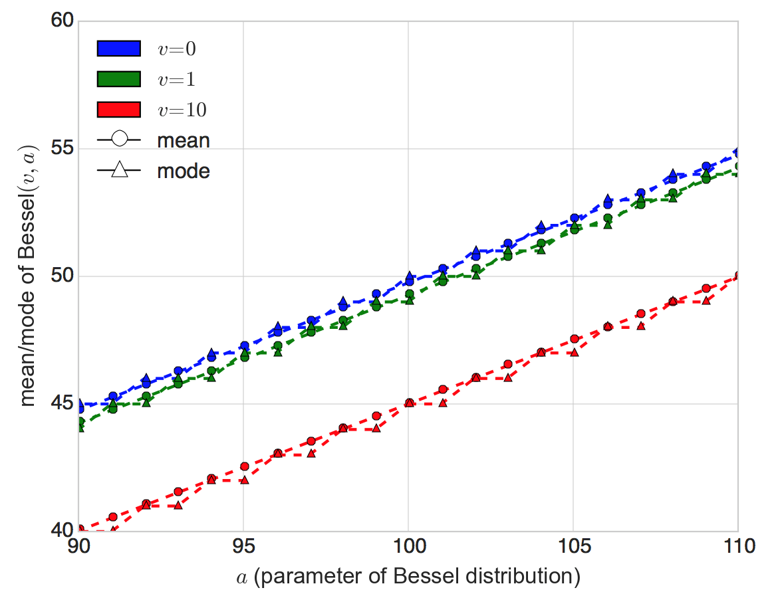
\includegraphics[width=0.6\textwidth]{figures/besselmode}
    \caption{Several comparisons of the mode versus the mean of the Bessel
    distribution. Each color represents a choice of $\nu$, with shapes of
    markers denoting the mode versus the mean.}
    \label{fig:besselmode}
  \end{figure}

  We empirically observe that the value of the expectation and the mode of a
  Bessel distribution are close. Figure \ref{fig:besselmode} shows that, though
  the mode is integer-valued while the mean is continuous, these quantities
  remain close across different parameter values of $\nu$ and $\alpha$. We can
  even provide a theoretical bound for the error between these two, which we
  prove in a third proposition:

  \begin{proposition} (Proven in appendix.) The absolute
  difference between the mean and mode of the Bessel distribution is bounded by
  1:
    \[ \big| \mathbbm{E}_{\Bess{m; \nu, a})}[m]  - \textup{mode} \left(\Bess{m;
    a, \nu} \right) \big|  \leq 1. \]
  \end{proposition}

  This choice allows a closed-form solution for the optimal variational
  distribution over $\yvtP$, where the expectation $\Eq{\ytP}$ is now
  deterministically computed from $\ms$ and $\ytPM$:
  \begin{equation}
  \label{eqn:opt-multi}
  Q^*(\yvtP) = \textup{Multinom} \biggl(\yvtP;\, \Eq{\ytP}, \left(\Gq{\lamP}, \Gq{\mu_{\subs 1}}, \dots, \Gq{\mu_{\subs K}} \right) \biggr).
  \end{equation}
  
  % In our case, we can consider the two-dimensional Poisson matrix factorization
  % where $\subs$ are represented by row $d$ and column $v$. We therefore
  % have
  % \begin{align}
  % \Eq{\ln \mu_{dv}} &= \Eq{\ln\left(\sum_{k=1}^K \theta_{dk}\phi_{kv}\right)} \notag \\
  % &\approx \ln\left(\Eq{\sum_{k=1}^K \theta_{dk}\phi_{kv}}\right)
  %  - \frac{\mathbbm{V}_{Q}\left[\sum_{k=1}^K \theta_{dk} \phi_{kv}\right]}{2 \, \left(\Eq{\sum_{k=1}^K \theta_{dk} \phi_{kv}}\right)^2} \notag \\
  % &=\ln\left(\sum_{k=1}^K \Eq{\theta_{dk}}\Eq{\phi_{kv}}\right)
  %  - \frac{\sum_{k=1}^K \Vq{\theta_{dk} \phi_{kv}}}{2 \, \left(\sum_{k=1}^K \Eq{\theta_{dk}} \Eq{\phi_{kv}}\right)^2}.
  % \end{align}
  % Finally, because $\theta_{dk}$ and $\phi_{kv}$ are independent, we have
  % \begin{align}
  % \Vq{\theta_{dk} \phi_{kv}} =& \Vq{\theta_{dk}} \Vq{\phi_{kv}} + \Vq{\theta_{dk}} \left(\Eq{\phi_{kv}}\right)^2 + \Vq{\phi_{kv}} \left(\Eq{\theta_{dk}}\right)^2.
  % \end{align}
  
  Using the new variational distributions from Equations \ref{eqn:opt} and
  \ref{eqn:opt-multi} in conjunction with the distributions offered by Equation
  \ref{eqn:caviopt} for the remaining variables, we can derive parameter updates
  for a full CAVI algorithm. We can compute the evidence lower bound (ELBO) as
  an augmentation of the ELBO for non-private Bayesian Poisson factorization
  inference. However, due to the steps taken above to replace the Bessel
  distribution with a point estimate and to approximate the geometric
  expectations in Equations \ref{eqn:geomterm_1}--\ref{eqn:geomterm_2}, the ELBO
  no longer necessarily monotonically increases throughout inference. In
  practice, we find that within the first 5 initial iterations in all our
  experiments, the ELBO stabilizes and then proceeds to monotonically increase.
  We verify convergence by also measuring the mean average error (MAE) from the
  true parameters in synthetic experiments and the original data in real data
  experiments.
  
  \section{Validation}
  \label{sec:validation}

  In order to test this result, we generated synthetic count data using a
  Poisson matrix factorization formulation analogous to the LDA topic model
  \citep{blei2003latent} with $D$ documents, $V$ unique terms in a document
  vocabulary, and $K$ latent topics. We first used a Gamma prior to generate two
  matrices of latent parameters, $\theta$ of dimension $D \times K$ and $\phi$
  of dimension $K \times V$. We then compute the product of these, $\theta \phi
  = \Yten$, as the Poisson prior of our data generation process. Finally, we add
  two-sided geometric noise scaled to $\epsilon / N = 1$, a ratio that applies
  when the privacy budget $\epsilon$ and the maximum allowed difference between
  documents $N$ are equal (e.g., a privacy budget of 2 to privatize 2-word
  spans). We then test our inference procedure to see how closely it estimates
  the true parameters of the original model. We find that our model successfully
  converges to within a reasonable estimate of the true model parameters given
  the data, as demonstrated in a small example in Figure \ref{fig:test_output}.

  \begin{table}[t]
    \center
    \small
    \begin{tabular}{|l|r|r|}
      \hline
      Method & Iterations & MAE \\
      \hline
      \Naive~MCMC & 5000 burnin + 1000 & 0.396 \\
      Private MCMC & 3000 burnin + 1000 & 0.208 \\
      Private MCMC & 2000 burnin + 1000 & 0.224 \\
      \hline 
      \Naive~VI & 42 & 0.492 \\
      \Naive~VI & 100 & 0.465 \\
      Private VI & 42 (converged) & 0.396 \\
      \hline
      Private MCMC, VI init & 1000 burnin + 1000 & 0.223 \\
      Private MCMC, VI init & 2000 burnin + 1000 & 0.208 \\
      \hline
    \end{tabular}
    \vspace{0.2cm}
    \caption{MAE over estimates of the Poisson model parameters inferred over
    the same 1000-by-1000 matrix with 50 latent components and noise scaled to
    $\epsilon/N = 1$. MCMC results used the algorithm from
    \cite{schein2018locally} were averaged over 10 samples taken 100 iterations
    apart after burnin. \TODO{Rerun VI entries, add plot showing convergence vs
    wall clock}}
    \label{tab:results_synth}
  \end{table}

  \begin{table}[t]
    \center
    \resizebox{\textwidth}{!}{%
    \small
    \begin{tabular}{|p{1.3in}|r p{4.2in}|}
      \hline
      Nonprivate with true data
      & 1  & \#\#\# year billion dollars budget million fiscal tax program expenditures \\
      & 2  & people education jobs american life workers work better million good \\
      \multirow{2}{1in}{40 iterations, MAE = 0.0897}
      & 3 & new children energy environment america help schools school technology science \\
      & 4 & health care work security insurance people make social welfare americans \\    
      \hline

      \Naive~VI
      & 1  & year billion dollars federal budget programs fiscal government million program \\
      & 2  & work people americans children make help let america need know \\
      \multirow{2}{1in}{52 iterations, MAE = 0.0157}
      & 3 & congress act energy states national program legislation economic america law \\
      & 4 & health care new congress year insurance medical americans legislation government \\     
      \hline

      Private VI
      & 1 & \#\#\# year million fiscal billion dollars years budget increase expenditures \\
      & 2 & know work children welfare people year reform new believe america \\
      \multirow{2}{1in}{100 iterations, MAE = 0.0157}
      & 3 & government congress energy federal national act states new policy program \\
      & 4 & health care government federal public security insurance congress new make \\
      \hline
    \end{tabular}}
    \vspace{0.2cm}
    \caption{Sample topics from 20-topic models of Enron inferred using our VI
    inference methods with privacy set to $\epsilon/N = 2$. \TODO{REDO WITH ENRON TEXT}}
    \label{tab:results_topics}
  \end{table}

  Using a larger example of a synthetic 1000-by-1000 matrix of count
  observations, we test the performance of this algorithm as compared to the
  performance using inference with MCMC \citep{schein2018locally}. We observe
  that a single-threaded version of the code from the MCMC implementation, even
  with optimizations such as reducing the frequency of parameter resampling for
  the noise distributions, each iteration of inference takes approximately 0.8
  seconds. Using 4000 iterations of burnin and 1000 to collect samples with 32
  cores, we are able to take the combined inference time down to 5 minutes
  (using 160 minutes of observed CPU time). In contrast, our variational
  inference model takes approximately 2.8 seconds per iteration, and requires
  only 41-42 iterations to converge across ten trials, resulting in a combined 1
  minute of inference (16 minutes of observed CPU time). Depending on the
  parallelization available, this method offers a 5-10x speedup over the fast
  inference method. This improvement should increase significantly as the size
  of the observed data increases.


  To evaluate our synthetic data experiments, we compare estimates of the true
  Poisson parameters $\mus$ used to generate our synthetic data and the inferred
  parameters of each model. We measure fit using the MAE of inferred Poisson
  parameters from the true parameters. We compare the existing MCMC algorithm
  and our new variational inference algorithm, with a baseline for each being
  the output of a model in which it is assumed no random noise was given (termed
  the ``\naive'' model).
  
  The result of these synthetic experiments are shown in Table
  \ref{tab:results_synth}. We observe that our informed VI approach performs
  similarly to a \naive~MCMC approach, i.e., one in which the model is unaware of
  the addition of two-sided geometric noise. In investigating, we find this to
  be a consequence of a common result of variational inference, in which the
  variance is underestimated \cite{blei2017variational}.

  To demonstrate that this model can learn interesting patterns on larger scale
  data, we also consider topic output for a topic model. We display topic model
  results in Table \ref{tab:results_topics} using a sample of 10,000 documents
  from the EnronSent dataset \cite{styler2011enronsent}.
  Again, we find that our model incorrectly estimates variance, producing
  results worse than \naive~variational inference. However, if we perform
  inference with an overestimate of the private noise, we can produce much
  better topics than the \naive~method. We even observe that this allows some
  regularization effect, as the resulting MAE is lower than on a model learned
  directly on the nonprivate data.

  \section{Discussion}
  We present a new CAVI algorithm for inference of Bayesian Poisson
  factorization models under local privacy. Our method relies on two key
  theoretical insights about the Bessel distribution: first, that with fixed
  $\nu$, it belongs to the exponential family, and second, that its mode is an
  integer neighbor of its mean. Using these, we implement a tool with
  significant performance improvements over even an optimized version of the
  prior MCMC algorithm. On a synthetic test case of inferring a rank-50
  factorization of an 1000 by 1000 data observation matrix, we obtain a 10x
  speedup in model inference over convergence of the MCMC method. Though the
  standard version of our privacy-aware method produces error similar to the
  \naive, non-private implementation of MCMC Bayesian Poisson factorization, we
  can produce improved results by overestimating the amount of private noise
  that was added, forcing additional sparsity into the model. Further, we can
  use this VI procedure as initialization for an MCMC model to improve
  performance.
  
  \bibliographystyle{plainnat}
  \bibliography{neurips_2019}
  
\end{document}
